%
% LOCAL DB
%
\sub{Datenspeicherung}
\todo{Cachen der Assets geht erst nach dem Build -> ServiceWorker}\autoref{chap:aufbau}\\
Redux Offline speichert, wie in \autoref{sub:reduxpersist} bereits beschrieben, alle im Redux Store verwalteten Daten im LocalStorage. \autoref{fig:local-rdx} zeigt alle gespeicherten, nutzerInnengenerierten Daten im LocalStorage.
%
\begin{figure}[H]
  \centering
  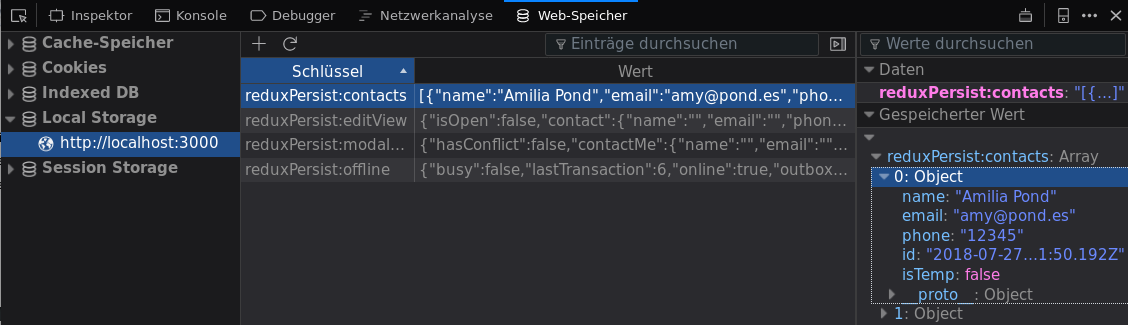
\includegraphics[width=\textwidth]{impl/localRdx}
  \grayRule
  \caption[Gespeicherte Daten im LocalStorage]{Gespeicherte Daten des Prototypen \it{amilia-rdx} im LocalStorage,\\Screenhot: Developer Tools im Firefox Browser}
  \label{fig:local-rdx}
\end{figure}
% 
Der Prototyp \it{amilia-qouch} nutzt zur lokalen Datenspeicherung PouchDB. PouchDB speichert die von NutzerInnen generierten Daten in IndexedDB, vgl. \autoref{chap:pouch}. In \autoref{fig:local-qouch} sind die gespeicherten Daten in der IndexedDB zu sehen.
%
\begin{figure}[H]
  \centering
  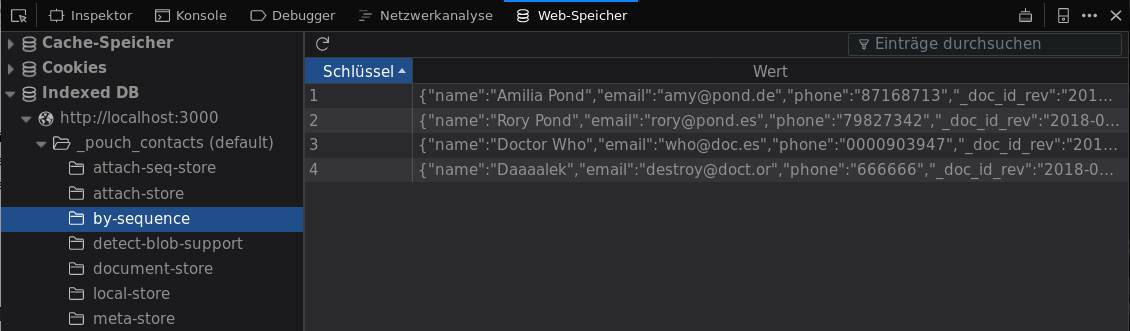
\includegraphics[width=\textwidth]{impl/localQouch}
  \grayRule
  \caption[Gespeicherte Daten in IndexedDB]{Gespeicherte Daten des Prototypen aus \it{amilia-qouch} in IndexedDB,\\Screenhot: Developer Tools im Firefox Browser}
  \label{fig:local-qouch}
\end{figure}
%
% SYNC
%
\sub{Datenbanksynchronisation}
Zwischen PouchDB und CouchDB können Daten in Echtzeit synchronisiert werden. Um die Live--Replikation zu aktivieren, muss im Synchronisationsaufruf der Parameter \tt{live: true} gesetzt sein.
Bricht die Internetverbindung ab, stoppt auch die Synchronisation.
Dank der angegebenen Parameter \tt{retry: true} versucht PouchDB die Synchronisation solange neuzustarten bis die Anwendung wieder mit dem Internet verbunden ist. \autoref{code:sync} zeigt die Implementation der Datenbankensynchronisation im Prototypen \it{amilia-qouch}.
%
\begin{center}
  \lstinputlisting[language=REACT,
  numbers=left,xleftmargin=20pt,
  firstline=1,lastline=5,
  framexleftmargin=15pt,
  caption={Synchronisation zwischen PouchDB und CouchDB im Prototyp \it{amilia-qouch}},
  label=code:sync]{code/sync.js}
\end{center}
Redux Offline nimmt einem auch Arbeit bei der Datensynchronisation ab. Alle Daten die sich im Queue befinden werden automatisch an den Server gesendet, sobald eine Internetverbindung besteht. Das funktioniert jedoch nicht so einfach wenn der Server nicht an ist. In der Dokumentation von Redux Offline steht, dass die Aktion solange versucht wird auszuführen, bis die Anwendung wieder mit dem Internet verbunden ist ~\cite{giving-up}. Allerdings wird die \sc{rollback} Aktion gefeuert wenn der Server nicht verfügbar ist und die Aktion wird abgebrochen.
\begin{center}
  \lstinputlisting[language=REACT,
  numbers=left,xleftmargin=20pt,
  firstline=6,
  framexleftmargin=15pt,
  caption={Discard Konfiguration für amilia-rdx},
  label=code:discard]{code/sync.js}
\end{center}
Die Discard Konfiguration bestimmt wann eine Aktion abgebrochen, und wann sie immer wieder neugestartet wird. Im \autoref{code:discard} ist in den Zeilen 1 bis 4 abzulesen wie diese Konfiguration überschrieben wird. Nun wird die Aktion nur abgebrochen wenn der Server verfügbar ist und einen \gls{HTTP} Status zwischen 400 und 500 zurückgibt.
In den darauffolgenden Zeilen wird die eigens implementierte Konfiguration mit der Standardkonfiguration von Redux Offline zusammengeführt wird.
Alle Daten werden nun auch nach einem Ausfall an den Server gesendet.\\
Im Gegensatz zum \it{amilia-qouch} Prototypen werden die Daten nur in eine Richtung automatisch gesendet. Es gibt keine Implementierung einer automatischen Replikation von den Daten auf dem Server zum lokalen Speicher.